\section{Software Design}
Software design is an important phase in software development process that lays foundation for building a well-structured and functional software systems. 
It outlines a strategy to transform the requirements of the application defined in \autoref{chap:requirements} into a well-defined and structured application.
As the project follows the MVVM architectural pattern, the application is divided into three components: \emph{model}, \emph{view}, \emph{view model}. 

\subsection{Model}
The \emph{model} represents the business logic to solve the problems listed as the requirements of the systems. Once the use cases outlined in \autoref{chap:requirements} are analyzed, the functions of each system components can be determined and then a sequence of operations can be created for each specific use case.
To gain a better overview and understanding of the entities inside the system, a diagram is created.
\begin{figure}[H]
    \centering
    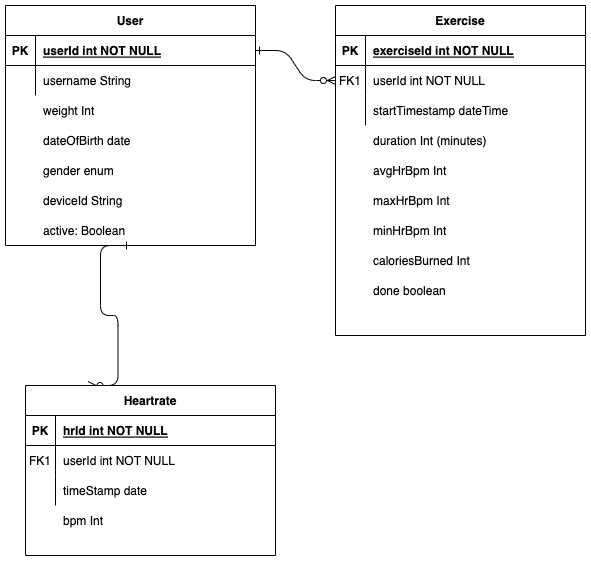
\includegraphics[width=0.8\textwidth]{diagrams/ham-entity.drawio.png}
    \caption{Entity class diagram}
    \label{fig:entity_diagram}
\end{figure}
This diagram illustrates the main entities and its relationship with each other inside the system. As described by the diagram, the main entities in the system consist of \emph{user}, \emph{exercise}, \emph{heartrate}. 
Each \emph{user} within the system has one to many relationship with both \emph{heartrate} and \emph{exercise} entities. These relationships represent the connection between a \emph{user} and their corresponding \emph{heartrate} and \emph{exercise} records. 
Once the entities have been defined, the system's functionalities can now be discussed based on the identified use cases.

\subsection{View}
\subsection{ViewModel}